% answers.tex —— 2009 年·普通高等学校招生考试·安徽卷·理科 · 参考答案与详细解析片段
% 由 tools/generate_projects.py 依来源总账自 2009/2009_数学真题_安徽理_试题.md + 2009/2009_数学真题_安徽理_解析正文.md + 2009/2009_数学真题_安徽理_答案要点.md 生成，勿手改（改源 MD 后重跑）


\begin{gktip}
固定候选 PDF 仅含题面，无答案、解析和评分标准，原卷亦未标分值；以下为非官方编者独立推导，官方答案字段为空。题面文字层只作定位，分数、根号、上下标与四幅图均以 600 dpi 原页复核。
\end{gktip}

\begin{answer}
\gksolhead{1}{}

\textbf{题目}：

$\mathrm i$ 是虚数单位，若 $\dfrac{1+7\mathrm i}{2-\mathrm i}=a+b\mathrm i$（$a,b\in\mathbf R$），则乘积 $ab$ 的值是（　）

（A）$-15$

（B）$-3$

（C）$3$

（D）$15$

\Needspace{4\baselineskip}
\textbf{解析}

\nopagebreak[4]
\[\frac{1+7\mathrm i}{2-\mathrm i}
=\frac{(1+7\mathrm i)(2+\mathrm i)}{(2-\mathrm i)(2+\mathrm i)}
=\frac{2+\mathrm i+14\mathrm i+7\mathrm i^2}{5}
=\frac{-5+15\mathrm i}{5}=-1+3\mathrm i .\]

故 $a=-1$、$b=3$，$ab=-3$，选 B。

\gkanswer{答案：B。}

\end{answer}
\begin{answer}
\gksolhead{2}{}

\textbf{题目}：

若集合 $A=\{x\mid |2x-1|<3\}$，$B=\left\{x\mid \dfrac{2x+1}{3-x}<0\right\}$，则 $A\cap B$ 是（　）

（A）$\left\{x\mid -1<x<-\dfrac12\ \text{\text{或}}\ 2<x<3\right\}$

（B）$\{x\mid 2<x<3\}$

（C）$\left\{x\mid -\dfrac12<x<2\right\}$

（D）$\left\{x\mid -1<x<-\dfrac12\right\}$

\Needspace{4\baselineskip}
\textbf{解析}

\nopagebreak[4]
\[|2x-1|<3\iff -3<2x-1<3\iff -1<x<2,\]

\Needspace{5\baselineskip}
故 $A=(-1,2)$。

\nopagebreak[4]
\[\frac{2x+1}{3-x}<0\iff (2x+1)(3-x)<0
\iff 2\left(x+\frac12\right)(3-x)<0 .\]

\Needspace{5\baselineskip}
两根为 $-\frac12$ 与 $3$，二次项系数为负，故解集为两侧：

\nopagebreak[4]
\[B=\left(-\infty,-\frac12\right)\cup(3,+\infty).\]

\Needspace{5\baselineskip}
于是

\nopagebreak[4]
\[A\cap B=\left(-1,-\frac12\right),\]

选 D。

\gkanswer{答案：D。}

\end{answer}
\begin{answer}
\gksolhead{3}{}

\textbf{题目}：

下列曲线中离心率为 $\dfrac{\sqrt6}{2}$ 的是（　）

（A）$\frac{x^2}{2}-\frac{y^2}{4}=1$

（B）$\frac{x^2}{4}-\frac{y^2}{2}=1$

（C）$\frac{x^2}{4}-\frac{y^2}{6}=1$

（D）$\frac{x^2}{4}-\frac{y^2}{10}=1$

\Needspace{4\baselineskip}
\textbf{解析}

对 $\frac{x^2}{a^2}-\frac{y^2}{b^2}=1$ 有 $e^2=1+\frac{b^2}{a^2}$，由 $e=\frac{\sqrt6}{2}$ 得 $e^2=\frac32$，故 $b^2=\frac12a^2$。

逐项检验：

\begin{itemize}
\item (A) $a^2=2$、$b^2=4$，$e^2=1+2=3$；
\item (B) $a^2=4$、$b^2=2$，$e^2=1+\frac12=\frac32$；
\item (C) $a^2=4$、$b^2=6$，$e^2=1+\frac32=\frac52$；
\item (D) $a^2=4$、$b^2=10$，$e^2=1+\frac52=\frac72$。
\end{itemize}

只有 (B) 符合，选 B。

\gkanswer{答案：B。}

\end{answer}
\begin{answer}
\gksolhead{4}{}

\textbf{题目}：

下列选项中，$p$ 是 $q$ 的必要不充分条件的是（　）

（A）$p:a+c>b+d$，$q:a>b$ 且 $c>d$

（B）$p:a>1$，$b>1$，$q:f(x)=a^x-b$（$a>0$，$a\neq1$）的图象不过第二象限

（C）$p:x=1$，$q:x^2=x$

（D）$p:a>1$，$q:f(x)=\log_a x$（$a>0$，$a\neq1$）在 $(0,+\infty)$ 上为增函数

\Needspace{4\baselineskip}
\textbf{解析}

「$p$ 是 $q$ 的必要不充分条件」要求 $q\Rightarrow p$ 且 $p\not\Rightarrow q$。

(A) 若 $a>b$ 且 $c>d$，两式相加得 $a+c>b+d$，故 $q\Rightarrow p$；反之取 $a=1$、$b=2$、$c=5$、$d=0$，有 $a+c=6>b+d=2$ 而 $a>b$ 不成立，故 $p\not\Rightarrow q$。符合。

(B) $a>1$、$b>1$ 时 $f(0)=1-b<0$，且 $f$ 在 $\mathbf R$ 上递增，故 $x<0$ 时 $f(x)<f(0)<0$，图象不过第二象限，即 $p\Rightarrow q$；反之由 $f$ 不过第二象限只能得 $a>1$ 与 $1-b\geqslant0$，推不出 $b>1$。故 $p$ 是充分不必要条件。

(C) $x=1\Rightarrow x^2=x$，故 $p$ 是充分不必要条件。

(D) $f(x)=\log_a x$ 在 $(0,+\infty)$ 上递增 $\iff a>1$，故为充要条件。

选 A。

\gkanswer{答案：A。}

\end{answer}
\begin{answer}
\gksolhead{5}{}

\textbf{题目}：

已知 $\{a_n\}$ 为等差数列，$a_1+a_3+a_5=105$，$a_2+a_4+a_6=99$，以 $S_n$ 表示 $\{a_n\}$ 的前 $n$ 项和，则使得 $S_n$ 达到最大值的 $n$ 是（　）

（A）$21$

（B）$20$

（C）$19$

（D）$18$

\Needspace{4\baselineskip}
\textbf{解析}

\nopagebreak[4]
\[a_1+a_3+a_5=3a_3=105\ \Longrightarrow\ a_3=35,\]

\nopagebreak[4]
\[a_2+a_4+a_6=3a_4=99\ \Longrightarrow\ a_4=33 .\]

\Needspace{5\baselineskip}
故公差 $d=a_4-a_3=-2$，

\nopagebreak[4]
\[a_n=a_3+(n-3)d=35-2(n-3)=41-2n .\]

由 $a_n\geqslant0$ 得 $n\leqslant20.5$，即 $a_{20}=1>0$、$a_{21}=-1<0$，故 $S_n$ 在 $n=20$ 时取最大值，选 B。

\gkanswer{答案：B。}

\end{answer}
\begin{answer}
\gksolhead{6}{}

\textbf{题目}：

设 $a<b$，函数 $y=(x-a)^2(x-b)$ 的图象可能是（　）
\nopagebreak[4]
\begin{center}% 2009 年安徽卷理科第 6 题：y=(x-a)^2(x-b)（a<b）的四个候选图象。
% 来源 PDF：普通高考/2009/2009安徽理.pdf，SHA256 e3986483e52654337c383d27cbe67e80ee0bd62eaf64defba6fe8bcc0cdb0c6d
% 原页：第 1 页（A3 三栏）第 2 栏上部，印刷页 495。
% 重绘依据：与同年安徽文科第 8 题同题同图，四幅小图 2×2 排布；(A) 与 x 轴有三个不同交点；
%   (B) 在 b 处相切、开口向下；(C) 在 a 处相切（局部极大为 0）、在 b 处自下而上穿过；(D) 在 b 处相切、局部极小为 0。
\begin{tikzpicture}[semithick, every node/.style={inner sep=1.1pt, font=\small}]
  % ---------- (A) ----------
  \begin{scope}[shift={(0,0)}, x=0.62cm, y=0.62cm]
    \begin{scope}
      \clip (-1.35,-2.35) rectangle (3.55,2.35);
      \draw[domain=-1.15:3.4,samples=200,smooth,variable=\x]
        plot (\x, {0.7*(-(\x+0.5))*(\x-0.35)*(\x-2.2)});
    \end{scope}
    \draw[-{Stealth}] (-1.3,0) -- (3.5,0) node[right] {$x$};
    \draw[-{Stealth}] (0,-2.25) -- (0,2.25) node[above] {$y$};
    \node[anchor=north east] at (-0.06,-0.08) {$O$};
    \node[below] at (0.75,-0.06) {$a$};
    \node[below] at (2.2,-0.06) {$b$};
    \node at (1.2,-3.05) {(A)};
  \end{scope}
  % ---------- (B) ----------
  \begin{scope}[shift={(5.0,0)}, x=0.62cm, y=0.62cm]
    \begin{scope}
      \clip (-1.35,-2.35) rectangle (3.55,2.35);
      \draw[domain=-1.15:3.4,samples=200,smooth,variable=\x]
        plot (\x, {0.7*(-(\x-0.35))*(\x-2.2)*(\x-2.2)});
    \end{scope}
    \draw[-{Stealth}] (-1.3,0) -- (3.5,0) node[right] {$x$};
    \draw[-{Stealth}] (0,-2.25) -- (0,2.25) node[above] {$y$};
    \node[anchor=north east] at (-0.06,-0.08) {$O$};
    \node[below] at (0.75,-0.06) {$a$};
    \node[below] at (2.2,-0.06) {$b$};
    \node at (1.2,-3.05) {(B)};
  \end{scope}
  % ---------- (C) ----------
  \begin{scope}[shift={(0,-4.2)}, x=0.62cm, y=0.62cm]
    \begin{scope}
      \clip (-1.35,-2.35) rectangle (3.55,2.35);
      \draw[domain=-1.15:3.4,samples=200,smooth,variable=\x]
        plot (\x, {0.7*(\x-0.35)*(\x-0.35)*(\x-2.2)});
    \end{scope}
    \draw[-{Stealth}] (-1.3,0) -- (3.5,0) node[right] {$x$};
    \draw[-{Stealth}] (0,-2.25) -- (0,2.25) node[above] {$y$};
    \node[anchor=north east] at (-0.06,-0.08) {$O$};
    \node[below] at (0.75,-0.06) {$a$};
    \node[below] at (2.2,-0.06) {$b$};
    \node at (1.2,-3.05) {(C)};
  \end{scope}
  % ---------- (D) ----------
  \begin{scope}[shift={(5.0,-4.2)}, x=0.62cm, y=0.62cm]
    \begin{scope}
      \clip (-1.35,-2.35) rectangle (3.55,2.35);
      \draw[domain=-1.15:3.4,samples=200,smooth,variable=\x]
        plot (\x, {0.7*(\x-0.35)*(\x-2.2)*(\x-2.2)});
    \end{scope}
    \draw[-{Stealth}] (-1.3,0) -- (3.5,0) node[right] {$x$};
    \draw[-{Stealth}] (0,-2.25) -- (0,2.25) node[above] {$y$};
    \node[anchor=north east] at (-0.06,-0.08) {$O$};
    \node[below] at (0.75,-0.06) {$a$};
    \node[below] at (2.2,-0.06) {$b$};
    \node at (1.2,-3.05) {(D)};
  \end{scope}
\end{tikzpicture}
\end{center}
\nopagebreak[4]
\Needspace{4\baselineskip}
\textbf{解析}

设 $f(x)=(x-a)^2(x-b)$，$a<b$。因 $(x-a)^2\geqslant0$：

\begin{itemize}
\item $x<b$ 时 $f(x)\leqslant0$，等号仅在 $x=a$ 处成立，即图象在 $x=a$ 处与 $x$ 轴相切，且该点为局部极大值 $0$；
\item $x>b$ 时 $f(x)>0$，即图象在 $x=b$ 处自下而上穿过 $x$ 轴；
\item 在 $a<x<b$ 上 $f<0$，极小值点为 $x=\frac{a+2b}{3}$；
\item $x\to-\infty$ 时 $f\to-\infty$，$x\to+\infty$ 时 $f\to+\infty$。
\end{itemize}

逐一对照：(A) 与 $x$ 轴有三个不同交点；(B) 在 $b$ 处相切且 $x\to+\infty$ 时 $f\to-\infty$；(D) 在 $a$ 处穿过、在 $b$ 处相切。只有 (C) 符合，选 C。

\gkanswer{答案：C。}

\end{answer}
\begin{answer}
\gksolhead{7}{}

\textbf{题目}：

若不等式组 $\begin{cases}x\geqslant0,\\ x+3y\geqslant4,\\ 3x+y\leqslant4\end{cases}$ 所表示的平面区域被直线 $y=kx+\dfrac43$ 分为面积相等的两部分，则 $k$ 的值是（　）

（A）$\frac73$

（B）$\frac37$

（C）$\frac43$

（D）$\frac34$

\Needspace{4\baselineskip}
\textbf{解析}

可行域为三角形，顶点为 $\left(0,\frac43\right)$、$(0,4)$、$(1,1)$。

\Needspace{5\baselineskip}
直线 $y=kx+\frac43$ 过顶点 $\left(0,\frac43\right)$，把三角形分成两个三角形。两部分面积相等，当且仅当该直线经过对边的中点，即 $(0,4)$ 与 $(1,1)$ 的中点

\nopagebreak[4]
\[M\left(\frac12,\frac52\right).\]

\Needspace{5\baselineskip}
故

\nopagebreak[4]
\[k=\frac{\frac52-\frac43}{\frac12-0}=\frac{7/6}{1/2}=\frac73,\]

选 A。

\gkanswer{答案：A。}

\end{answer}
\begin{answer}
\gksolhead{8}{}

\textbf{题目}：

已知函数 $f(x)=\sqrt3\sin\omega x+\cos\omega x$（$\omega>0$），$y=f(x)$ 的图象与直线 $y=2$ 的两个相邻交点的距离等于 $\pi$，则 $f(x)$ 的单调递增区间是（　）

（A）$\left[k\pi-\dfrac{\pi}{12},\ k\pi+\dfrac{5\pi}{12}\right]$，$k\in\mathbf Z$

（B）$\left[k\pi+\dfrac{5\pi}{12},\ k\pi+\dfrac{11\pi}{12}\right]$，$k\in\mathbf Z$

（C）$\left[k\pi-\dfrac{\pi}{3},\ k\pi+\dfrac{\pi}{6}\right]$，$k\in\mathbf Z$

（D）$\left[k\pi+\dfrac{\pi}{6},\ k\pi+\dfrac{2\pi}{3}\right]$，$k\in\mathbf Z$

\Needspace{4\baselineskip}
\textbf{解析}

\nopagebreak[4]
\[f(x)=\sqrt3\sin\omega x+\cos\omega x
=2\left(\frac{\sqrt3}{2}\sin\omega x+\frac12\cos\omega x\right)
=2\sin\left(\omega x+\frac\pi6\right).\]

\Needspace{5\baselineskip}
最大值为 $2$，故 $y=f(x)$ 与 $y=2$ 的交点就是图象的最高点；两相邻最高点的距离等于一个周期，于是

\nopagebreak[4]
\[\frac{2\pi}{\omega}=\pi\ \Longrightarrow\ \omega=2 .\]

\nopagebreak[4]
\[f(x)=2\sin\left(2x+\frac\pi6\right).\]

\Needspace{5\baselineskip}
递增需

\nopagebreak[4]
\[-\frac\pi2+2k\pi\leqslant 2x+\frac\pi6\leqslant\frac\pi2+2k\pi,\]

\Needspace{5\baselineskip}
解得

\nopagebreak[4]
\[k\pi-\frac\pi3\leqslant x\leqslant k\pi+\frac\pi6,\]

即单调递增区间为 $\left[k\pi-\frac{\pi}{3},k\pi+\frac{\pi}{6}\right]$，选 C。

\gkanswer{答案：C。}

\end{answer}
\begin{answer}
\gksolhead{9}{}

\textbf{题目}：

已知函数 $f(x)$ 在 $\mathbf R$ 上满足 $f(x)=2f(2-x)-x^2+8x-8$，则曲线 $y=f(x)$ 在点 $(1,f(1))$ 处的切线方程是（　）

（A）$y=2x-1$

（B）$y=x$

（C）$y=3x-2$

（D）$y=-2x+3$

\Needspace{4\baselineskip}
\textbf{解析}

\Needspace{5\baselineskip}
取 $x=1$：

\nopagebreak[4]
\[f(1)=2f(1)-1+8-8\ \Longrightarrow\ f(1)=1 .\]

\Needspace{5\baselineskip}
对 $f(x)=2f(2-x)-x^2+8x-8$ 两边求导：

\nopagebreak[4]
\[f'(x)=-2f'(2-x)-2x+8 .\]

\Needspace{5\baselineskip}
取 $x=1$：

\nopagebreak[4]
\[f'(1)=-2f'(1)-2+8\ \Longrightarrow\ 3f'(1)=6\ \Longrightarrow\ f'(1)=2 .\]

\Needspace{5\baselineskip}
故切线为

\nopagebreak[4]
\[y-1=2(x-1)\ \Longrightarrow\ y=2x-1,\]

选 A。

\gkanswer{答案：A。}

\end{answer}
\begin{answer}
\gksolhead{10}{}

\textbf{题目}：

考察正方体 $6$ 个面的中心，甲从这 $6$ 个点中任意选两个点连成直线，乙也从这 $6$ 个点中任意选两个点连成直线，则所得的两条直线相互平行但不重合的概率等于（　）

（A）$\frac1{75}$

（B）$\frac2{75}$

（C）$\frac3{75}$

（D）$\frac4{75}$

\Needspace{4\baselineskip}
\textbf{解析}

$6$ 个面心构成正八面体，任取两点连成直线共 $\mathrm C_6^2=15$ 条，其中 $12$ 条为棱（长 $\sqrt2$）、$3$ 条为过相对顶点的长对角线（长 $2$）。

对每一对坐标轴（共 $3$ 对），$4$ 条棱围成一个正方形，其中有 $2$ 组平行边；故平行的直线对共 $3\times2=6$ 组。三条长对角线两两不平行，也不与棱平行。

\Needspace{5\baselineskip}
甲、乙各选一条，共 $15\times15=225$ 种等可能结果。两直线平行但不重合即取自同一组平行线对，有序对数为 $6\times2=12$。故

\nopagebreak[4]
\[P=\frac{12}{225}=\frac{4}{75},\]

选 D。

\gkanswer{答案：D。}

\end{answer}
\begin{answer}
\gksolhead{11}{}

\textbf{题目}：

若随机变量 $X\sim N(\mu,\sigma^2)$，则 $P(X\leqslant\mu)=$\gkblank{}．

\Needspace{4\baselineskip}
\textbf{解析}

\Needspace{5\baselineskip}
正态密度曲线关于 $x=\mu$ 对称，故

\nopagebreak[4]
\[P(X\leqslant\mu)=P(X\geqslant\mu)=\frac12 .\]

\gkanswer{答案：$\frac12$。}

\end{answer}
\begin{answer}
\gksolhead{12}{}

\textbf{题目}：

以直角坐标系的原点为极点，$x$ 轴的正半轴为极轴，并在两种坐标系中取相同的长度单位．已知直线的极坐标方程为 $\theta=\dfrac{\pi}{4}$（$\rho\in\mathbf R$），它与曲线 $\begin{cases}x=1+2\cos\alpha,\\ y=2+2\sin\alpha\end{cases}$（$\alpha$ 为参数）相交于两点 $A$ 和 $B$，则 $|AB|=$\gkblank{}．

\Needspace{4\baselineskip}
\textbf{解析}

$\theta=\frac\pi4$（$\rho\in\mathbf R$）即直线 $y=x$。

\Needspace{5\baselineskip}
由 $\begin{cases}x=1+2\cos\alpha,\\ y=2+2\sin\alpha\end{cases}$ 消去参数：

\nopagebreak[4]
\[(x-1)^2+(y-2)^2=4,\]

是圆心 $(1,2)$、半径 $2$ 的圆。

\Needspace{5\baselineskip}
圆心到 $x-y=0$ 的距离

\nopagebreak[4]
\[d=\frac{|1-2|}{\sqrt2}=\frac1{\sqrt2},\]

\Needspace{5\baselineskip}
故

\nopagebreak[4]
\[|AB|=2\sqrt{r^2-d^2}=2\sqrt{4-\frac12}=\sqrt{14}.\]

\gkanswer{答案：$\sqrt{14}$。}

\end{answer}
\begin{answer}
\gksolhead{13}{}

\textbf{题目}：

程序框图（即算法流程图）如图所示，其输出结果是\gkblank{}．
\nopagebreak[4]
\begin{center}% 2009 年安徽卷理科第 13 题：程序框图，输出 a 的值。
% 来源 PDF：普通高考/2009/2009安徽理.pdf，SHA256 e3986483e52654337c383d27cbe67e80ee0bd62eaf64defba6fe8bcc0cdb0c6d
% 原页：第 1 页（A3 三栏）第 2 栏下部，印刷页 495。
% 重绘依据：开始 → a=1 → a=2a+1 → 判断 a>100；否（左）回到 a=2a+1，是（下）→ 输出 a → 结束。
\begin{tikzpicture}[scale=0.9, semithick, >=Stealth,
  node distance=5mm, every node/.style={inner sep=3pt, font=\small}]
  \node (start) [draw, rounded corners=4pt, minimum width=1.9cm, minimum height=0.62cm] {开始};
  \node (init) [draw, minimum width=1.9cm, minimum height=0.62cm, below=of start] {$a=1$};
  \node (step) [draw, minimum width=2.6cm, minimum height=0.62cm, below=of init] {$a=2a+1$};
  \node (cond) [draw, diamond, aspect=2.0, minimum width=2.6cm, minimum height=0.95cm, below=of step] {$a>100$};
  \node (out) [draw, trapezium, trapezium left angle=70, trapezium right angle=110,
    minimum width=2.4cm, minimum height=0.62cm, below=of cond] {输出 $a$};
  \node (end) [draw, rounded corners=4pt, minimum width=1.9cm, minimum height=0.62cm, below=of out] {结束};
  \draw[->] (start) -- (init);
  \draw[->] (init) -- (step);
  \draw[->] (step) -- (cond);
  \draw[->] (cond) -- (out);
  \node[anchor=west] at ($(cond.south)!0.5!(out.north)+(16pt,-4pt)$) {是};
  \draw[->] (cond.west) -- ++(-0.85,0) |- node[pos=0.25, left] {否} (step.west);
  \draw[->] (out) -- (end);
\end{tikzpicture}
\end{center}
\nopagebreak[4]
\Needspace{4\baselineskip}
\textbf{解析}

\Needspace{5\baselineskip}
初始 $a=1$，每次执行 $a\leftarrow2a+1$：

\nopagebreak[4]
\[1\to3\to7\to15\to31\to63\to127 .\]

当 $a=127>100$ 时跳出循环并输出 $127$。

\gkanswer{答案：$127$。}

\end{answer}
\begin{answer}
\gksolhead{14}{}

\textbf{题目}：

给定两个长度为 $1$ 的平面向量 $\overrightarrow{OA}$ 和 $\overrightarrow{OB}$，它们的夹角为 $120^\circ$，如图所示，点 $C$ 在以 $O$ 为圆心的圆弧 $AB$ 上变动．若 $\overrightarrow{OC}=x\overrightarrow{OA}+y\overrightarrow{OB}$，其中 $x,y\in\mathbf R$，则 $x+y$ 的最大值是\gkblank{}．
\nopagebreak[4]
\begin{center}% 2009 年安徽卷理科第 14 题：单位向量 OA、OB 夹角 120°，C 在圆弧 AB 上变动。
% 来源 PDF：普通高考/2009/2009安徽理.pdf，SHA256 e3986483e52654337c383d27cbe67e80ee0bd62eaf64defba6fe8bcc0cdb0c6d
% 原页：第 1 页（A3 三栏）第 3 栏上部，印刷页 495。
% 重绘依据：O 在左下，OA 水平向右，OB 与 OA 成 120°；以 O 为圆心、OA 为半径作从 B 到 A 的圆弧，
%   C 取在弧上，画向量 OC；OA、OB、OC 均为带箭头向量。
\begin{tikzpicture}[scale=0.95, semithick, >=Stealth, every node/.style={inner sep=1.4pt}]
  \coordinate (O) at (0,0);
  \coordinate (A) at (3,0);
  \coordinate (B) at (120:3);
  \coordinate (C) at (55:3);
  \draw (B) arc[start angle=120, end angle=0, radius=3];
  \draw[->] (O) -- (A);
  \draw[->] (O) -- (B);
  \draw[->] (O) -- (C);
  \fill (C) circle (1.1pt);
  \node[below left] at (O) {$O$};
  \node[below right] at (A) {$A$};
  \node[left] at (B) {$B$};
  \node[above right] at (C) {$C$};
\end{tikzpicture}
\end{center}
\nopagebreak[4]
\Needspace{4\baselineskip}
\textbf{解析}

\Needspace{5\baselineskip}
$C$ 在圆弧 $AB$ 上，故 $|\overrightarrow{OC}|=1$。由 $\overrightarrow{OC}=x\overrightarrow{OA}+y\overrightarrow{OB}$ 及

\nopagebreak[4]
\[|\overrightarrow{OA}|=|\overrightarrow{OB}|=1,\qquad
\overrightarrow{OA}\cdot\overrightarrow{OB}=\cos120^\circ=-\frac12,\]

\Needspace{5\baselineskip}
得

\nopagebreak[4]
\[1=x^2+y^2+2xy\left(-\frac12\right)=x^2+y^2-xy .\]

\Needspace{5\baselineskip}
记 $s=x+y$，则 $x^2+y^2=s^2-2xy$，代入得

\nopagebreak[4]
\[s^2-3xy=1\ \Longrightarrow\ xy=\frac{s^2-1}{3}.\]

\Needspace{5\baselineskip}
由 $x,y\in\mathbf R$ 需 $(x+y)^2\geqslant4xy$：

\nopagebreak[4]
\[s^2\geqslant\frac{4(s^2-1)}{3}\ \Longrightarrow\ 3s^2\geqslant4s^2-4\ \Longrightarrow\ s^2\leqslant4,\]

故 $s\leqslant2$。

当 $x=y=1$ 时 $\overrightarrow{OC}=\overrightarrow{OA}+\overrightarrow{OB}$，其模为 $2\cos60^\circ=1$，符合 $C$ 在圆弧上（此时 $C$ 为弧 $AB$ 的中点）。故 $x+y$ 的最大值为 $2$。

\gkanswer{答案：$2$。}

\end{answer}
\begin{answer}
\gksolhead{15}{}

\textbf{题目}：

对于四面体 $ABCD$，下列命题正确的是\gkblank{}．（写出所有正确命题的编号）

① 相对棱 $AB$ 与 $CD$ 所在的直线异面；

② 由顶点 $A$ 作四面体的高，其垂足是 $\triangle BCD$ 的三条高线的交点；

③ 若分别作 $\triangle ABC$ 和 $\triangle ABD$ 的边 $AB$ 上的高，则这两条高所在直线异面；

④ 分别作三组相对棱中点的连线，所得的三条线段相交于一点；

⑤ 最长棱必有某个端点，由它引出的另两条棱的长度之和大于最长棱．

\Needspace{4\baselineskip}
\textbf{解析}

① 正确：四面体中相对的两棱不共面，所在直线必异面。

② 错误：设 $A$ 在平面 $BCD$ 上的垂足为 $H$，则 $AH\perp$ 平面 $BCD$。由三垂线定理，$H$ 为 $\triangle BCD$ 的垂心需 $AB\perp CD$、$AC\perp BD$、$AD\perp BC$ 同时成立（垂心四面体），一般四面体不满足。

③ 错误：两条高都垂直于 $AB$，若垂足重合则两直线相交，不是异面直线。

④ 正确：设 $E,F$ 为 $AB,CD$ 中点，$G,H$ 为 $AC,BD$ 中点，$I,J$ 为 $AD,BC$ 中点，则三条线段 $EF$、$GH$、$IJ$ 都经过四面体重心并被其平分，故交于一点。

⑤ 正确：设 $AB$ 为最长棱，在 $\triangle ABC$ 中 $AC+BC>AB$，故端点 $A$（或 $B$）引出的两条棱之和大于 $AB$。

故填 ①④⑤。

\gkanswer{答案：①④⑤。}

\end{answer}
\begin{answer}
\gksolhead{16}{}

\textbf{题目}：

在 $\triangle ABC$ 中，$\sin(C-A)=1$，$\sin B=\dfrac13$．

（1）求 $\sin A$ 的值；

（2）设 $AC=\sqrt6$，求 $\triangle ABC$ 的面积．

\Needspace{4\baselineskip}
\textbf{解析}

\Needspace{5\baselineskip}
（1）由 $\sin(C-A)=1$ 及 $0<C-A<\pi$ 得

\nopagebreak[4]
\[C-A=\frac\pi2\ \Longrightarrow\ C=A+\frac\pi2 .\]

\Needspace{5\baselineskip}
于是

\nopagebreak[4]
\[B=\pi-A-C=\frac\pi2-2A,\]

\nopagebreak[4]
\[\sin B=\sin\left(\frac\pi2-2A\right)=\cos2A=1-2\sin^2A=\frac13,\]

\Needspace{5\baselineskip}
故

\nopagebreak[4]
\[\sin^2A=\frac13 .\]

\Needspace{5\baselineskip}
由 $B>0$ 得 $2A<\frac\pi2$，即 $A$ 为锐角，所以

\nopagebreak[4]
\[\sin A=\frac{\sqrt3}{3},\qquad \cos A=\sqrt{1-\frac13}=\frac{\sqrt6}{3}.\]

\Needspace{5\baselineskip}
（2）

\nopagebreak[4]
\[\sin C=\sin\left(A+\frac\pi2\right)=\cos A=\frac{\sqrt6}{3}.\]

\Needspace{5\baselineskip}
由正弦定理

\nopagebreak[4]
\[\frac{a}{\sin A}=\frac{b}{\sin B},\qquad b=AC=\sqrt6,\]

\Needspace{5\baselineskip}
得

\nopagebreak[4]
\[a=\sqrt6\cdot\frac{\sqrt3/3}{1/3}=3\sqrt2 .\]

\Needspace{5\baselineskip}
故

\nopagebreak[4]
\[S=\frac12ab\sin C=\frac12\cdot3\sqrt2\cdot\sqrt6\cdot\frac{\sqrt6}{3}=3\sqrt2 .\]

\gkanswer{答案：（1）$\dfrac{\sqrt3}{3}$；（2）$3\sqrt2$。}

\end{answer}
\begin{answer}
\gksolhead{17}{}

\textbf{题目}：

某地有 $A,B,C,D$ 四人先后感染了甲型 H1N1 流感，其中只有 $A$ 到过疫区．$B$ 肯定是受 $A$ 感染的．对于 $C$，因为难以断定他是受 $A$ 还是受 $B$ 感染的，于是假定他受 $A$ 和受 $B$ 感染的概率都是 $\dfrac12$．同样也假定 $D$ 受 $A$、$B$ 和 $C$ 感染的概率都是 $\dfrac13$．在这种假定之下，$B$、$C$、$D$ 中直接受 $A$ 感染的人数 $X$ 就是一个随机变量．写出 $X$ 的分布列（不要求写出计算过程），并求 $X$ 的均值（即数学期望）．

\Needspace{4\baselineskip}
\textbf{解析}

$B$ 必直接受 $A$ 感染；$C$ 直接受 $A$ 感染的概率为 $\frac12$；$D$ 直接受 $A$ 感染的概率为 $\frac13$。三人是否直接受 $A$ 感染相互独立。

\Needspace{5\baselineskip}
故 $X=1+Y+Z$，其中 $Y\sim B\left(1,\frac12\right)$、$Z\sim B\left(1,\frac13\right)$，$X$ 的可能取值为 $1,2,3$。

\nopagebreak[4]
\[P(X=1)=P(Y=0)P(Z=0)=\frac12\cdot\frac23=\frac13,\]

\nopagebreak[4]
\[P(X=2)=P(Y=1)P(Z=0)+P(Y=0)P(Z=1)
=\frac12\cdot\frac23+\frac12\cdot\frac13=\frac12,\]

\nopagebreak[4]
\[P(X=3)=P(Y=1)P(Z=1)=\frac12\cdot\frac13=\frac16 .\]

分布列：

\begin{center}
\begin{tabular}{llll}
\toprule
$X$ & 1 & 2 & 3 \\
\midrule
$P$ & $\frac13$ & $\frac12$ & $\frac16$ \\
\bottomrule
\end{tabular}
\end{center}

\nopagebreak[4]
\[EX=1\cdot\frac13+2\cdot\frac12+3\cdot\frac16
=\frac13+1+\frac12=\frac{11}{6}.\]

（也可用 $EX=1+EY+EZ=1+\frac12+\frac13=\frac{11}{6}$。）

\gkanswer{答案：$P(X=1)=\frac13$，$P(X=2)=\frac12$，$P(X=3)=\frac16$；$EX=\frac{11}{6}$。}

\end{answer}
\begin{answer}
\gksolhead{18}{}

\textbf{题目}：

如图，四棱锥 $F-ABCD$ 的底面 $ABCD$ 是菱形，其对角线 $AC=2$，$BD=\sqrt2$，$AE$、$CF$ 都与平面 $ABCD$ 垂直，$AE=1$，$CF=2$．

（1）求二面角 $B-AF-D$ 的大小；

（2）求四棱锥 $E-ABCD$ 与四棱锥 $F-ABCD$ 公共部分的体积．
\nopagebreak[4]
\begin{center}% 2009 年安徽卷理科第 18 题：四棱锥 F-ABCD 与四棱锥 E-ABCD 共底。
% 来源 PDF：普通高考/2009/2009安徽理.pdf，SHA256 e3986483e52654337c383d27cbe67e80ee0bd62eaf64defba6fe8bcc0cdb0c6d
% 原页：第 2 页（A3 三栏）第 1 栏上部，印刷页 496。
% 重绘依据：按原图菱形 ABCD 以斜投影画出，A 在左、D 在前下、C 在右、B 在后方（被遮挡）；
%   E 在 A 正上方、F 在 C 正上方，AE、CF 竖直；FA、FD、FC 与 AD、DC 实线，
%   AB、BC、BF 因被遮挡画虚线。
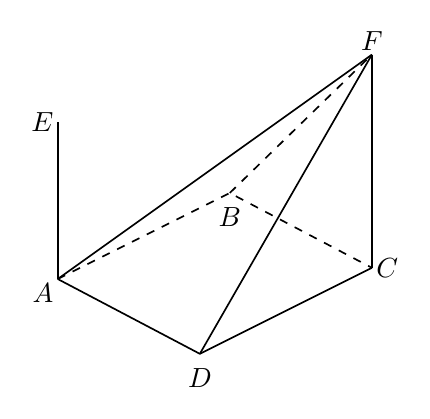
\begin{tikzpicture}[scale=0.95, semithick, every node/.style={inner sep=1.3pt}]
  \coordinate (A) at (0,0);
  \coordinate (D) at (1.9,-1.0);
  \coordinate (C) at (4.2,0.15);
  \coordinate (B) at (2.3,1.15);
  \coordinate (E) at (0,2.1);
  \coordinate (F) at (4.2,3.0);
  % 底面
  \draw (A) -- (D) -- (C);
  \draw[dashed] (A) -- (B) -- (C);
  % 侧棱
  \draw (A) -- (F);
  \draw (D) -- (F);
  \draw (C) -- (F);
  \draw[dashed] (B) -- (F);
  % 竖直棱
  \draw (A) -- (E);
  \node[below left] at (A) {$A$};
  \node[below] at ([yshift=-4pt]D) {$D$};
  \node[right] at (C) {$C$};
  \node[anchor=north] at ([yshift=-4pt]B) {$B$};
  \node[left] at (E) {$E$};
  \node[above] at (F) {$F$};
\end{tikzpicture}
\end{center}
\nopagebreak[4]
\Needspace{4\baselineskip}
\textbf{解析}

\Needspace{5\baselineskip}
以菱形中心 $O$ 为原点，$AC$ 为 $x$ 轴、$BD$ 为 $y$ 轴，平面 $ABCD$ 为 $z=0$。由 $AC=2$、$BD=\sqrt2$：

\nopagebreak[4]
\[A(-1,0,0),\quad C(1,0,0),\quad
B\left(0,\tfrac{\sqrt2}{2},0\right),\quad D\left(0,-\tfrac{\sqrt2}{2},0\right).\]

\Needspace{5\baselineskip}
$AE\perp$ 平面 $ABCD$、$CF\perp$ 平面 $ABCD$，且 $AE=1$、$CF=2$，故

\nopagebreak[4]
\[E(-1,0,1),\qquad F(1,0,2).\]

\Needspace{5\baselineskip}
（1）

\nopagebreak[4]
\[\overrightarrow{AB}=\left(1,\tfrac{\sqrt2}{2},0\right),\quad
\overrightarrow{AD}=\left(1,-\tfrac{\sqrt2}{2},0\right),\quad
\overrightarrow{AF}=(2,0,2).\]

\nopagebreak[4]
\[\boldsymbol n_1=\overrightarrow{AB}\times\overrightarrow{AF}
=\left(\tfrac{\sqrt2}{2}\cdot2,\ -(1\cdot2),\ 1\cdot0-\tfrac{\sqrt2}{2}\cdot2\right)
=(\sqrt2,-2,-\sqrt2),\]

\nopagebreak[4]
\[\boldsymbol n_2=\overrightarrow{AD}\times\overrightarrow{AF}
=\left(-\tfrac{\sqrt2}{2}\cdot2,\ -(1\cdot2),\ 0+\tfrac{\sqrt2}{2}\cdot2\right)
=(-\sqrt2,-2,\sqrt2).\]

\nopagebreak[4]
\[\boldsymbol n_1\cdot\boldsymbol n_2=-2+4-2=0,\]

故平面 $BAF\perp$ 平面 $DAF$，二面角 $B-AF-D$ 为 $90^\circ$。

（2）记 $z$ 为到平面 $ABCD$ 的距离（$0\leqslant z\leqslant1$）。

棱锥 $E-ABCD$ 的高为 $1$、顶点在 $A$ 的正上方，故高度 $z$ 处的截面是底面以 $A$ 为中心、比例 $1-z$ 的位似图形，即中心在 $(-z,0)$、两条半对角线为 $1-z$ 与 $\frac{\sqrt2}{2}(1-z)$ 的菱形。

棱锥 $F-ABCD$ 的高为 $2$、顶点在 $C$ 的正上方，高度 $z$ 处的截面是底面以 $C$ 为中心、比例 $1-\frac z2$ 的位似图形，即中心在 $\left(\frac z2,0\right)$、两条半对角线为 $1-\frac z2$ 与 $\frac{\sqrt2}{2}\left(1-\frac z2\right)$ 的菱形。

两个菱形同向、中心都在 $x$ 轴上。由于各边所在直线随 $z$ 线性移动，交集多边形的顶点坐标是 $z$ 的一次函数，故交集面积是 $z$ 的二次函数。

计算三个特殊高度：

\begin{itemize}
\item $z=0$：两截面都等于底面，$A(0)=\sqrt2$；
\item $z=\frac13$：第一个菱形半对角线缩为 $\frac23$ 与 $\frac{\sqrt2}{3}$，第二个缩为 $\frac56$ 与 $\frac{5\sqrt2}{12}$，交集为菱形，$A\left(\frac13\right)=\frac{\sqrt2}{4}$；
\item $z=\frac23$：第二个菱形的左顶点恰与第一个菱形的右顶点重合，交集退化为一点，$A\left(\frac23\right)=0$。
\end{itemize}

\Needspace{5\baselineskip}
由二次函数的三点式解得

\nopagebreak[4]
\[A(z)=\sqrt2\left(1-3z+\frac94z^2\right)\quad\left(0\leqslant z\leqslant\frac23\right),\]

且 $z>\frac23$ 时两截面不相交。

\Needspace{5\baselineskip}
故公共部分体积

\nopagebreak[4]
\[V=\int_0^{2/3}A(z)\,\mathrm dz
=\sqrt2\left[z-\frac32z^2+\frac34z^3\right]_0^{2/3}
=\sqrt2\left(\frac23-\frac23+\frac29\right)=\frac{2\sqrt2}{9}.\]

\Needspace{5\baselineskip}
\textbf{几何解释（可用于核对）}：直线 $AF$ 与 $EC$ 相交于点

\nopagebreak[4]
\[Q\left(-\frac13,0,\frac23\right),\]

\Needspace{5\baselineskip}
而以 $ABCD$ 为底、$Q$ 为顶点的四棱锥，其高度 $z$ 处的截面正是中心在 $\left(-\frac z2,0\right)$、水平半对角线为 $\frac{2-3z}{2}$ 的菱形，面积同样为

\nopagebreak[4]
\[\frac{\sqrt2}{4}(2-3z)^2 .\]

\Needspace{5\baselineskip}
两个立体同底且各个高度的截面面积相同，故公共部分就是该四棱锥，

\nopagebreak[4]
\[V=\frac13\cdot S_{ABCD}\cdot\frac23=\frac13\cdot\sqrt2\cdot\frac23=\frac{2\sqrt2}{9},\]

与积分结果一致。

\gkanswer{答案：（1）$90^\circ$；（2）$\dfrac{2\sqrt2}{9}$。}

\end{answer}
\begin{answer}
\gksolhead{19}{}

\textbf{题目}：

已知函数 $f(x)=x-\dfrac2x+a(2-\ln x)$，$a>0$．讨论 $f(x)$ 的单调性．

\Needspace{4\baselineskip}
\textbf{解析}

\Needspace{5\baselineskip}
定义域 $(0,+\infty)$，

\nopagebreak[4]
\[f'(x)=1+\frac{2}{x^2}-\frac ax=\frac{x^2-ax+2}{x^2}.\]

分子为二次式，判别式 $\Delta=a^2-8$。

\begin{itemize}
\item 当 $0<a\leqslant2\sqrt2$ 时，$\Delta\leqslant0$，分子恒非负，故 $f'(x)\geqslant0$，$f$ 在 $(0,+\infty)$ 上单调递增。
\item 当 $a>2\sqrt2$ 时，$\Delta>0$，方程 $x^2-ax+2=0$ 有两正根
\end{itemize}

\nopagebreak[4]
\[x_1=\frac{a-\sqrt{a^2-8}}{2},\qquad x_2=\frac{a+\sqrt{a^2-8}}{2},\qquad 0<x_1<x_2 .\]

$f'$ 在 $(0,x_1)$ 与 $(x_2,+\infty)$ 上为正，在 $(x_1,x_2)$ 上为负。故 $f$ 在 $(0,x_1)$、$(x_2,+\infty)$ 上递增，在 $(x_1,x_2)$ 上递减。

\gkanswer{答案：$0<a\leqslant2\sqrt2$ 时在 $(0,+\infty)$ 上单调递增；$a>2\sqrt2$ 时在 $\left(0,\frac{a-\sqrt{a^2-8}}2\right)$ 与 $\left(\frac{a+\sqrt{a^2-8}}2,+\infty\right)$ 上递增，在两者之间递减。}

\end{answer}
\begin{answer}
\gksolhead{20}{}

\textbf{题目}：

点 $P(x_0,y_0)$ 在椭圆 $\dfrac{x^2}{a^2}+\dfrac{y^2}{b^2}=1$（$a>b>0$）上，$x_0=a\cos\beta$，$y_0=b\sin\beta$，$0<\beta<\dfrac{\pi}{2}$．直线 $l_2$ 与直线 $l_1:\dfrac{x_0}{a^2}x+\dfrac{y_0}{b^2}y=1$ 垂直，$O$ 为坐标原点，直线 $OP$ 的倾斜角为 $\alpha$，直线 $l_2$ 的倾斜角为 $\gamma$．

（1）证明：点 $P$ 是椭圆 $\dfrac{x^2}{a^2}+\dfrac{y^2}{b^2}=1$ 与直线 $l_1$ 的唯一交点；

（2）证明：$\tan\alpha$，$\tan\beta$，$\tan\gamma$ 构成等比数列．

\Needspace{4\baselineskip}
\textbf{解析}

\Needspace{5\baselineskip}
（1）由 $x_0=a\cos\beta$、$y_0=b\sin\beta$ 得

\nopagebreak[4]
\[\frac{x_0^2}{a^2}+\frac{y_0^2}{b^2}=\cos^2\beta+\sin^2\beta=1,\]

\Needspace{5\baselineskip}
故 $P$ 在椭圆上。又

\nopagebreak[4]
\[\frac{x_0^2}{a^2}+\frac{y_0^2}{b^2}=1\]

说明 $P$ 也满足 $l_1$ 的方程 $\frac{x_0x}{a^2}+\frac{y_0y}{b^2}=1$。

\Needspace{5\baselineskip}
设 $(x,y)$ 是椭圆与 $l_1$ 的公共点。由柯西不等式

\nopagebreak[4]
\[1=\left(\frac{x_0x}{a^2}+\frac{y_0y}{b^2}\right)^2
\leqslant\left(\frac{x_0^2}{a^2}+\frac{y_0^2}{b^2}\right)\left(\frac{x^2}{a^2}+\frac{y^2}{b^2}\right)=1,\]

\Needspace{5\baselineskip}
等号成立需 $\left(\frac{x}{a},\frac{y}{b}\right)$ 与 $\left(\frac{x_0}{a},\frac{y_0}{b}\right)$ 成比例，设

\nopagebreak[4]
\[\frac xa=t\frac{x_0}{a},\qquad \frac yb=t\frac{y_0}{b}.\]

\Needspace{5\baselineskip}
代入 $l_1$：

\nopagebreak[4]
\[t\left(\frac{x_0^2}{a^2}+\frac{y_0^2}{b^2}\right)=1\ \Longrightarrow\ t=1,\]

故 $(x,y)=(x_0,y_0)$。即 $P$ 是唯一交点。

\Needspace{5\baselineskip}
（2）由 $P(a\cos\beta,b\sin\beta)$：

\nopagebreak[4]
\[\tan\alpha=\frac{b\sin\beta}{a\cos\beta}=\frac ba\tan\beta .\]

\Needspace{5\baselineskip}
$l_1$ 的斜率为

\nopagebreak[4]
\[k_1=-\frac{x_0/a^2}{y_0/b^2}
=-\frac{b^2x_0}{a^2y_0}
=-\frac{b^2\cdot a\cos\beta}{a^2\cdot b\sin\beta}
=-\frac ba\cot\beta .\]

\Needspace{5\baselineskip}
$l_2\perp l_1$，故

\nopagebreak[4]
\[\tan\gamma=-\frac{1}{k_1}=\frac ab\tan\beta .\]

\Needspace{5\baselineskip}
于是

\nopagebreak[4]
\[\tan\alpha\cdot\tan\gamma
=\frac ba\tan\beta\cdot\frac ab\tan\beta=\tan^2\beta,\]

且 $\tan\alpha,\tan\beta,\tan\gamma$ 均不为 $0$（因 $0<\beta<\frac\pi2$），故三者构成等比数列。

\gkanswer{答案：（1）（2）证明见解析。}

\end{answer}
\begin{answer}
\gksolhead{21}{}

\textbf{题目}：

首项为正数的数列 $\{a_n\}$ 满足 $a_{n+1}=\dfrac14\left(a_n^2+3\right)$，$n\in\mathbf N_+$．

（1）证明：若 $a_1$ 为奇数，则对一切 $n\geqslant2$，$a_n$ 都是奇数；

（2）若对一切 $n\in\mathbf N_+$ 都有 $a_{n+1}>a_n$，求 $a_1$ 的取值范围．

\Needspace{4\baselineskip}
\textbf{解析}

\Needspace{5\baselineskip}
（1）设 $a_k$ 为奇数，则 $a_k^2$ 为奇数，$a_k^2+3$ 为偶数。又奇数的平方除以 $8$ 余 $1$：

\nopagebreak[4]
\[a_k=2m+1\ \Longrightarrow\ a_k^2=4m(m+1)+1\equiv1\pmod 8,\]

\Needspace{5\baselineskip}
故 $a_k^2+3\equiv4\pmod 8$，即 $a_k^2+3$ 能被 $4$ 整除且

\nopagebreak[4]
\[\frac{a_k^2+3}{4}\equiv1\pmod2 .\]

于是 $a_{k+1}=\frac{a_k^2+3}{4}$ 为奇数。由归纳法，$a_1$ 为奇数时对一切 $n\geqslant2$，$a_n$ 都是奇数。

\Needspace{5\baselineskip}
（2）

\nopagebreak[4]
\[a_{n+1}-a_n=\frac{a_n^2+3}{4}-a_n=\frac{a_n^2-4a_n+3}{4}=\frac{(a_n-1)(a_n-3)}{4}.\]

\Needspace{5\baselineskip}
故

\nopagebreak[4]
\[a_{n+1}>a_n\iff a_n<1\ \text{\text{或}}\ a_n>3 .\]

逐段讨论（已知 $a_1>0$）：

\begin{itemize}
\item $0<a_1<1$：此时 $a_1^2<1$，故 $a_2=\frac{a_1^2+3}{4}<1$，且 $(a_1-1)(a_1-3)>0$，即 $a_2>a_1$。归纳得 $0<a_n<1$ 且数列递增，条件恒成立。
\item $a_1=1$：$a_2=\frac{1+3}{4}=1$，数列为常数列，不满足严格递增。
\item $1<a_1<3$：$(a_1-1)(a_1-3)<0$，故 $a_2<a_1$，不满足。
\item $a_1=3$：$a_2=3$，常数列，不满足。
\item $a_1>3$：$a_1^2>9$，故 $a_2=\frac{a_1^2+3}{4}>3$，且 $(a_1-1)(a_1-3)>0$ 给出 $a_2>a_1$。归纳得 $a_n>3$ 且数列递增，条件恒成立。
\end{itemize}

综上，$a_1\in(0,1)\cup(3,+\infty)$。

\gkanswer{答案：（1）证明见解析；（2）$0<a_1<1$ 或 $a_1>3$。}

\end{answer}